\chapter{Packing the robot}
\label{chap:packing}   

In this section, the necessary steps for preparing the robot for shipment are described. Please consult the photos in this section for details.
A checklist of the material that you should take along in the robot shipping box in order to properly pack the robot is listed at \footnote{\url{https://raw.github.com/ipa320/setup/master/manual_ipa/ShippingBox.pdf}}.
Moreover, you should also always travel with a ''first-aid'' box that allows you to address common problems that may arise with the robot. The checklist for this first-aid box is listed at \footnote{\url{https://raw.github.com/ipa320/setup/master/manual_ipa/FirstAidKit.pdf}}.

The necessary packing steps are as follows:
\begin{itemize}
\item {\em Prepare the box.} Take out everything that could be in the way. Lay the tension belt flat on the ramp or under it. Open the front door (snap-on magnet). Remove the {\bf 2} rear cover from the robot.
\item {\em Drive the robot into the box.} Take care that the robot is centered in the box as much as possible. Make sure that the black marks are free and there are some centimeters to the board of the lower belts.
\item {\em Push emergency stop button, then power off.} {\bf Attention:} Always push the emergency button before turning power off. Otherwise, the torso may lose its reference position, requiring a lenghty recalibration process.
\item {\em Fasten the robot with a tension belt, but not too hard!} {\bf Attention:} Make sure the fastener or the tension belt is not in contact with the robot cover. 
\item {\em Use foam material to protect the robot and to prevent slipping.} Make sure that no part of the robot is in contact with the tension belts and the robot hast a good safty distance all around to the box. 
\item {\em Air travle} For air travel, fix an additional tension belt around the box. Moreover, seal the hinges with a plastic seal.
\end{itemize}

\newpage

\begin{figure}[!ht]
%\centering
\mbox{\subfigure{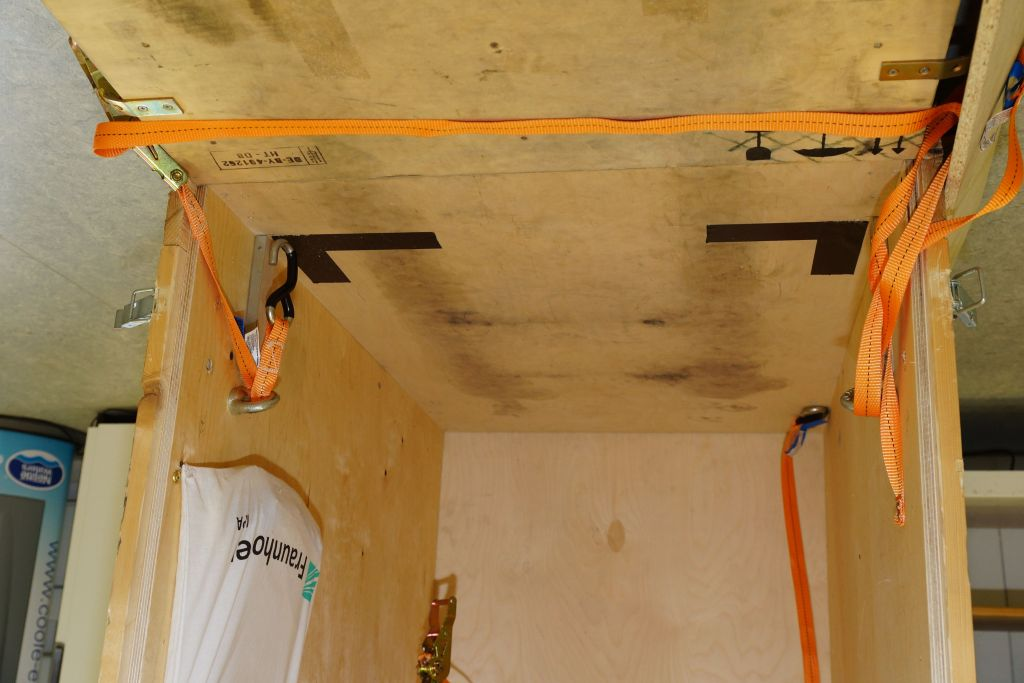
\includegraphics[width=7cm,angle=180]{images/packing_01.jpg}}\quad
\subfigure{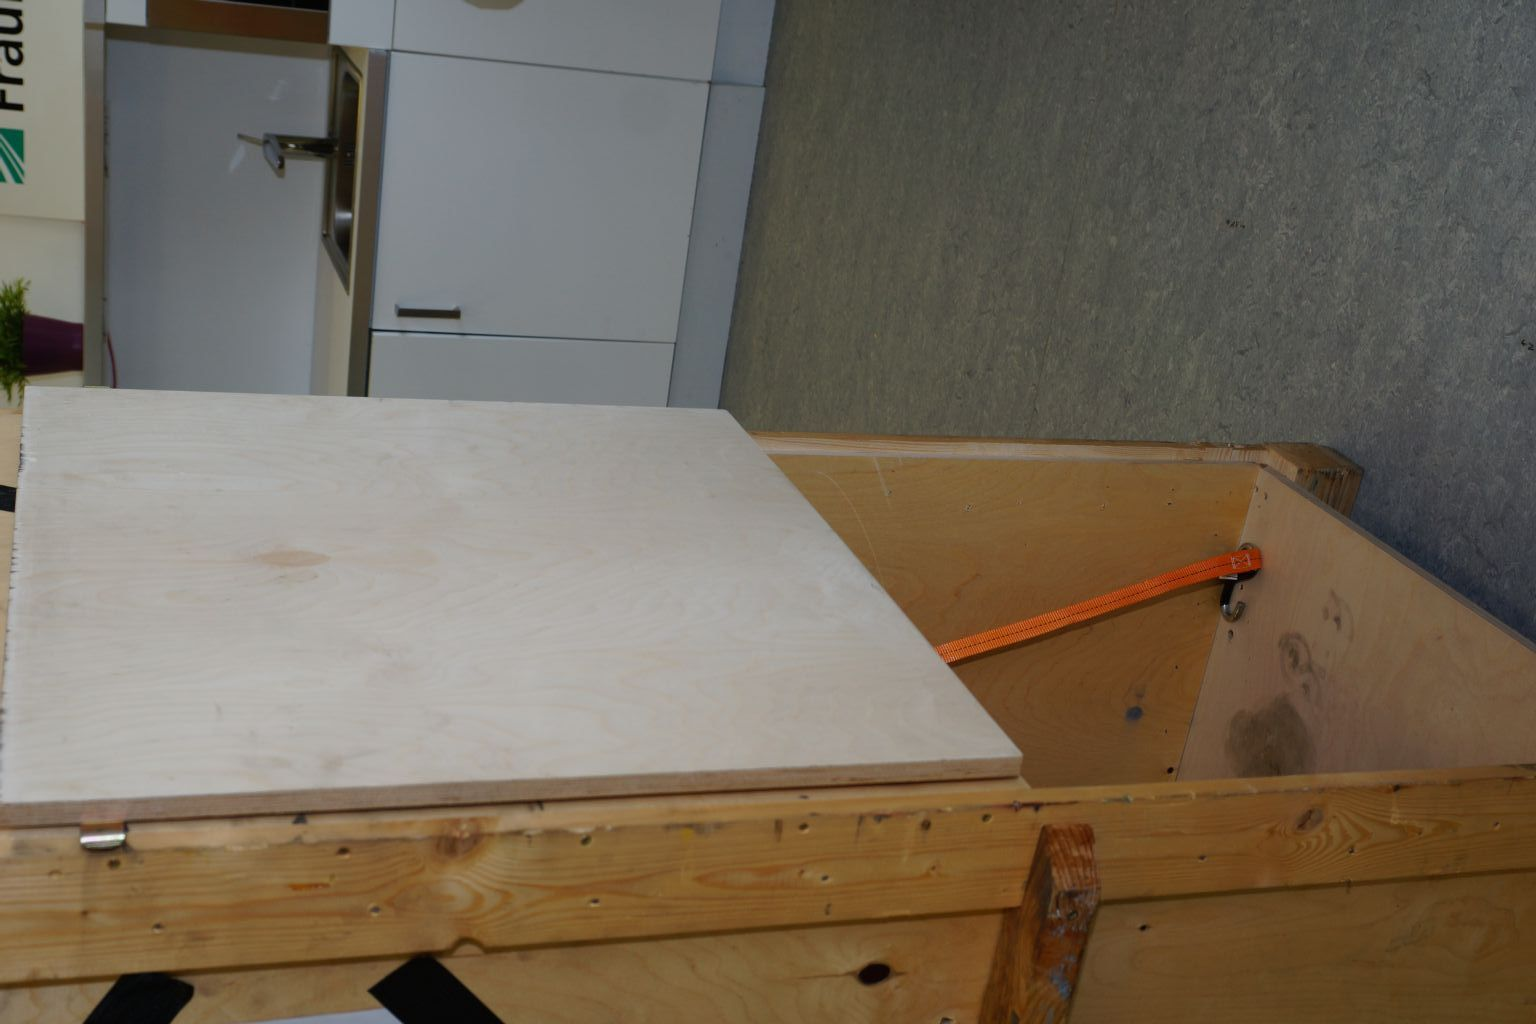
\includegraphics[width=7cm,angle=270]{images/packing_02.jpg} }}
\caption{Step 0: Remove board and put the belt aside (left). Open the front door (right).} % \label{fig12}
\end{figure}

\begin{figure}[!ht]
\centering
\mbox{\subfigure{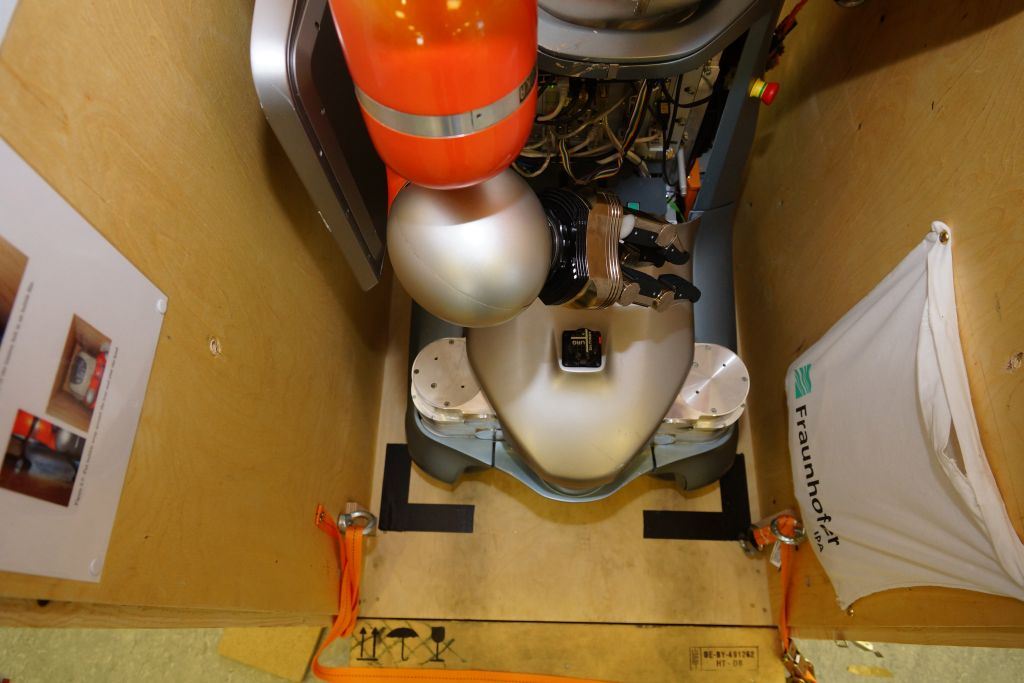
\includegraphics[width=7cm]{images/packing_03.jpg}}\quad
\subfigure{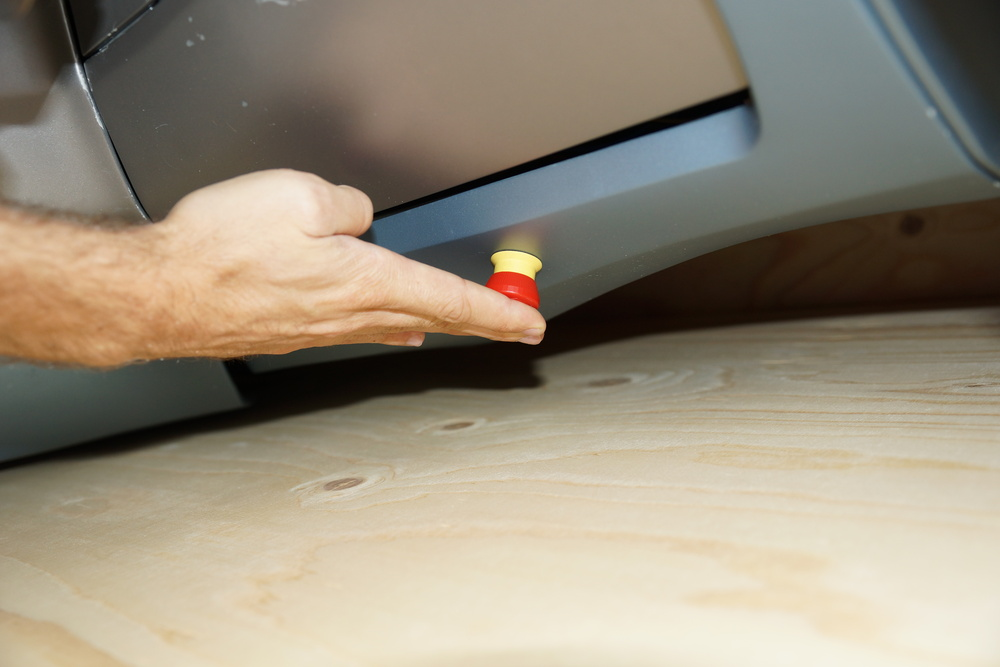
\includegraphics[width=7cm,angle=90]{images/packing_04.jpg} }}
\caption{Step 1: Drive the robot in the box and park it as centrally as possible (left). {\bf Always push the emergency stop button before power off!}} % \label{fig12} 
\end{figure}

\begin{figure}[!ht]
\centering
\mbox{\subfigure{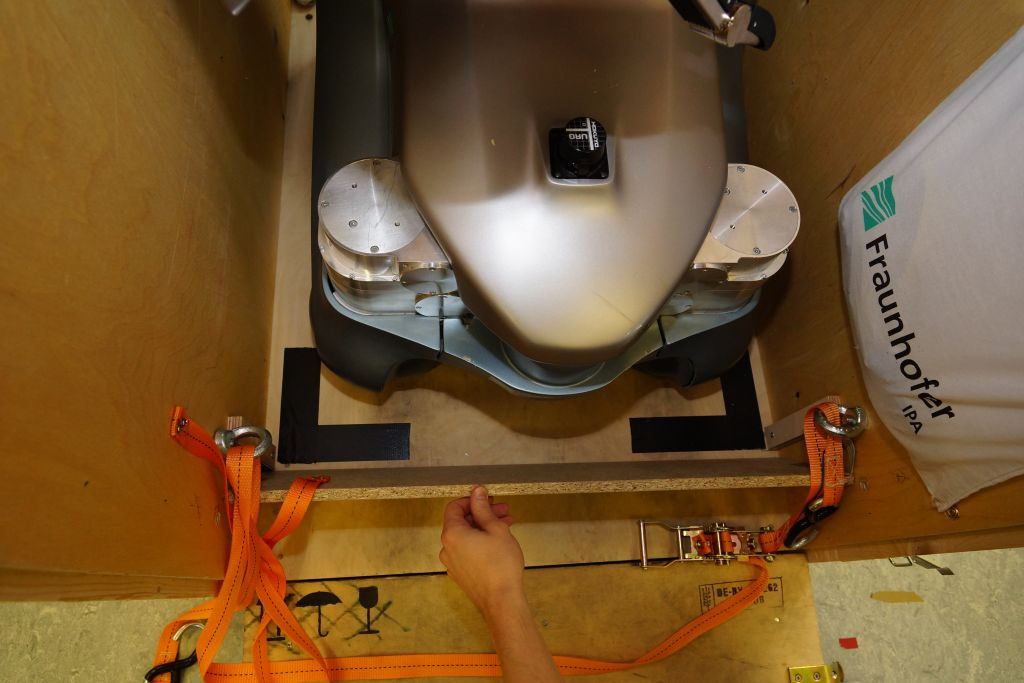
\includegraphics[width=7cm]{images/packing_05.jpg}}\quad
\subfigure{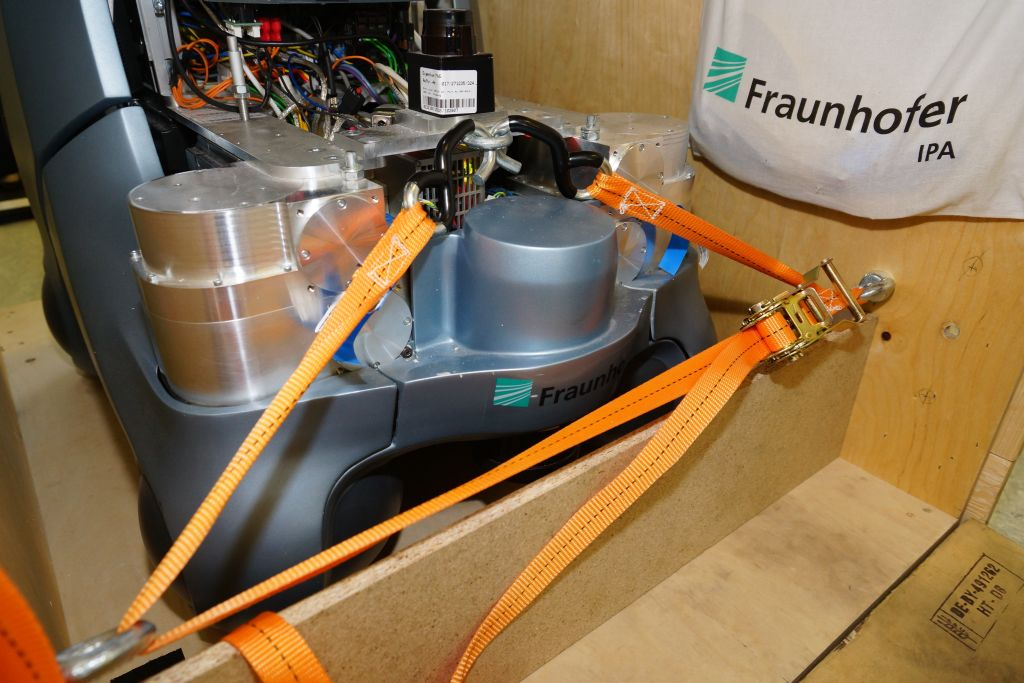
\includegraphics[width=7cm]{images/packing_06.jpg} }}
\caption{Step 2: Place the borad under the lower belts (left). Hook in the ends of the belt and fasten it \bf{moderatly} (right).} % \label{fig12} 
\end{figure}

\begin{figure}[!ht]
\centering
\mbox{\subfigure{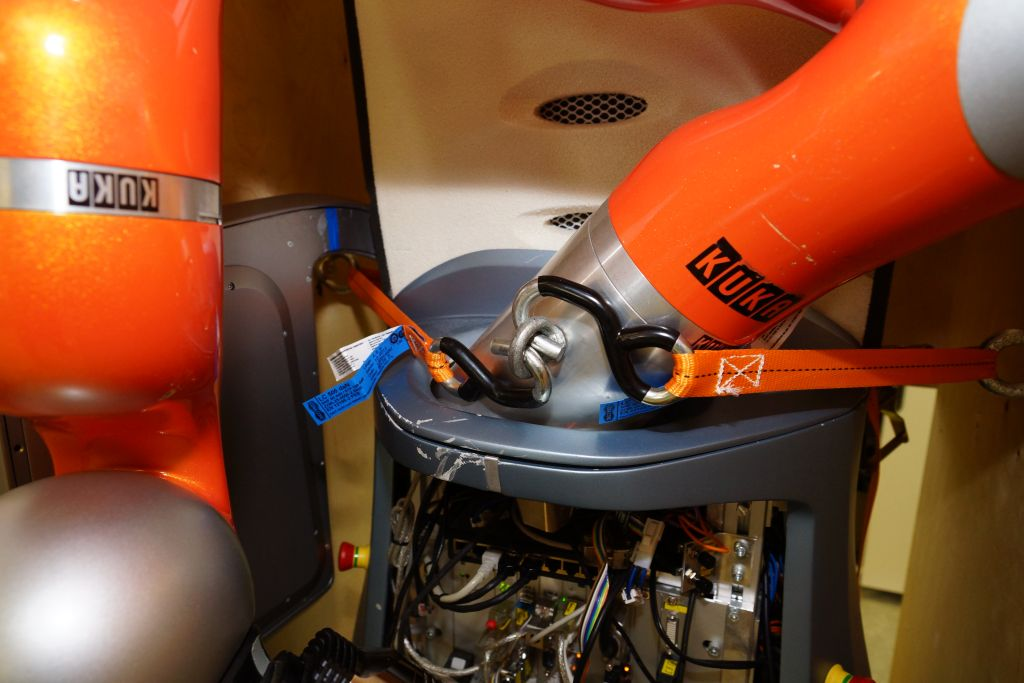
\includegraphics[width=7cm]{images/packing_07.jpg}}\quad
\subfigure{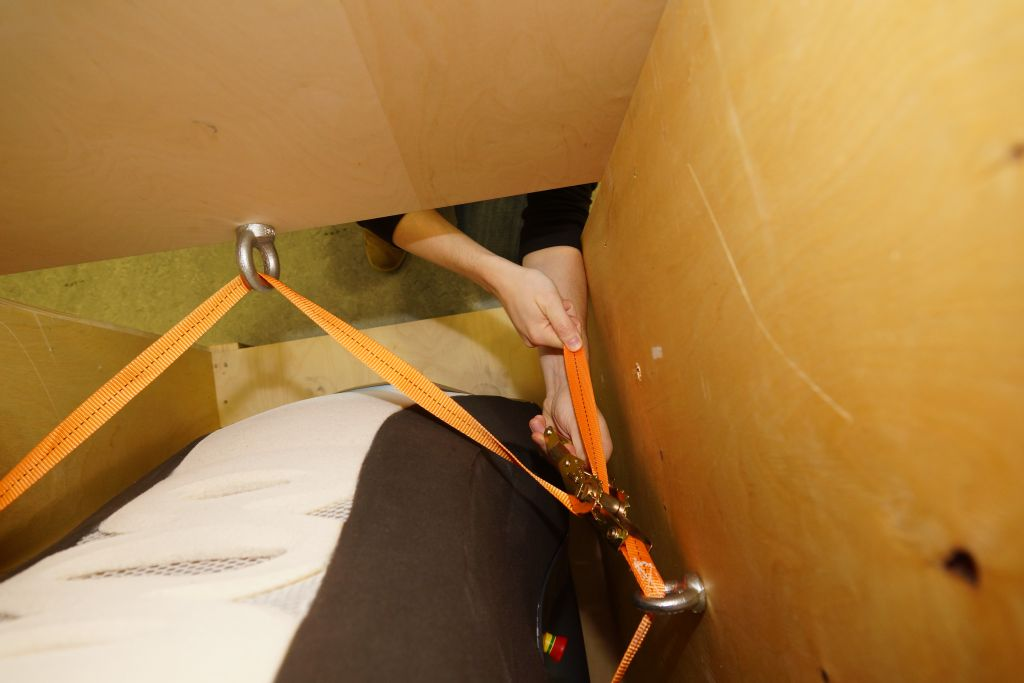
\includegraphics[width=7cm]{images/packing_08.jpg} }}
\caption{Step 3: Hook in the ends of the upper belt (left). Fasten the belt from the front (right).} % \label{fig12} 
\end{figure}

\begin{figure}[!ht]
\centering
\mbox{\subfigure{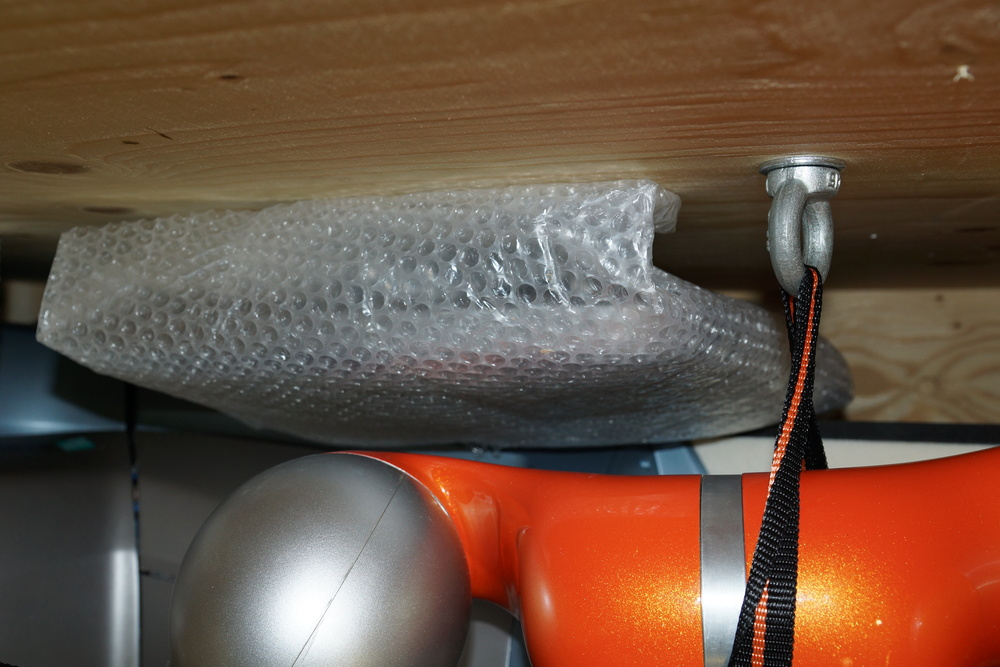
\includegraphics[width=8cm, angle=90]{images/packing_09.jpg}}\quad
\subfigure{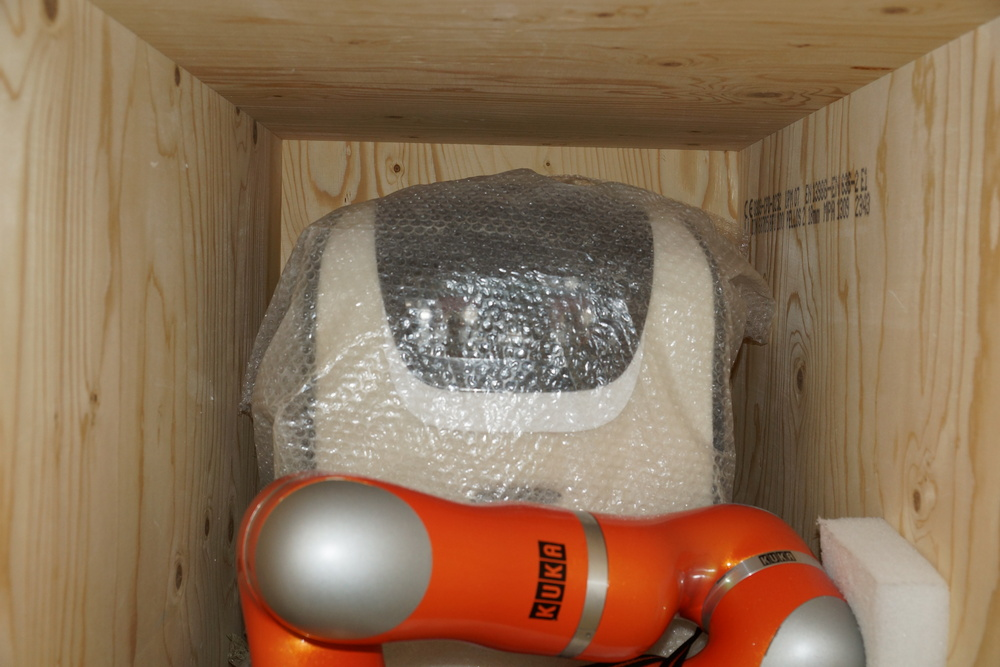
\includegraphics[width=7cm]{images/packing_10.jpg} }}
\caption{Step 4: Put bubble wrap around the tray and over the head.} %\label{fig12}
\end{figure}

\begin{figure}[!ht]
\centering
\mbox{\subfigure{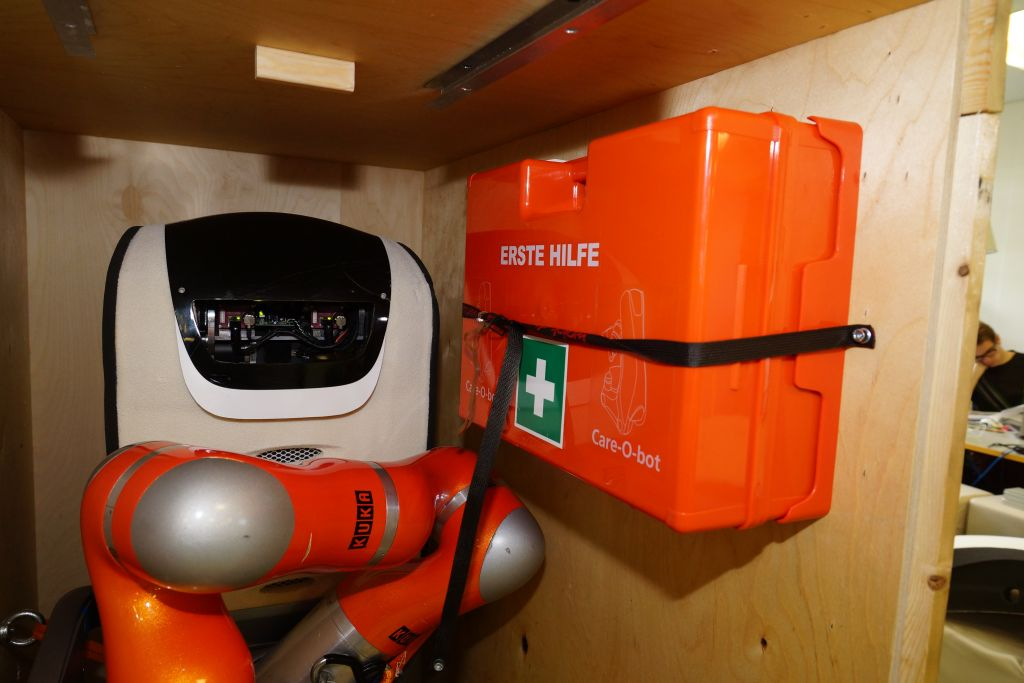
\includegraphics[width=7cm]{images/packing_11.jpg}}\quad
\subfigure{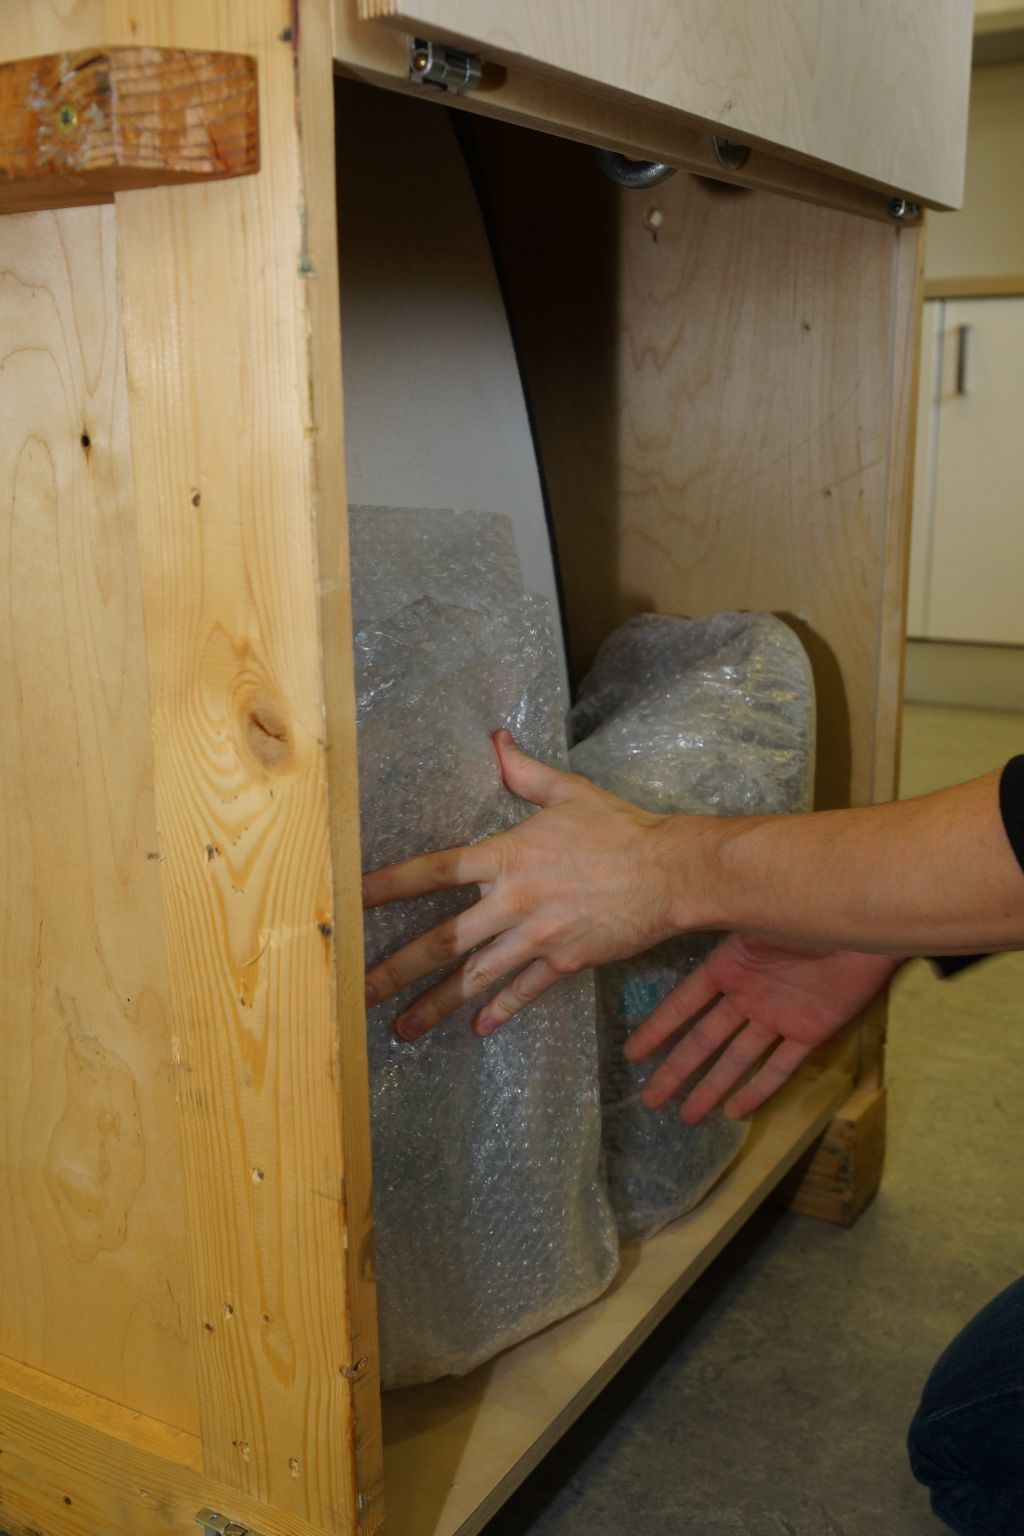
\includegraphics[width=6cm,angle=0]{images/packing_12.jpg} }}
\caption{Step 5: Put the ''first-aid'' box in holder and fasten the strap (left). Wrap the rear covers in bubble foil an put it infront of the robot. (right).} % \label{fig12} 
\end{figure}

\begin{figure}[!ht]
\centering
\mbox{\subfigure{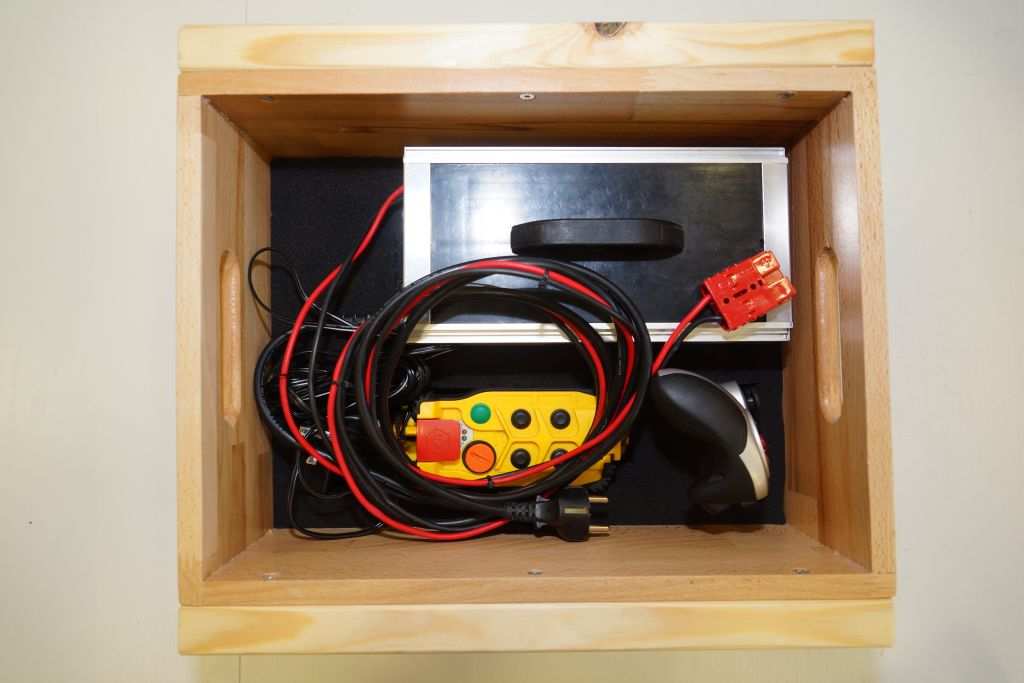
\includegraphics[width=7cm]{images/packing_13.jpg}}\quad
\subfigure{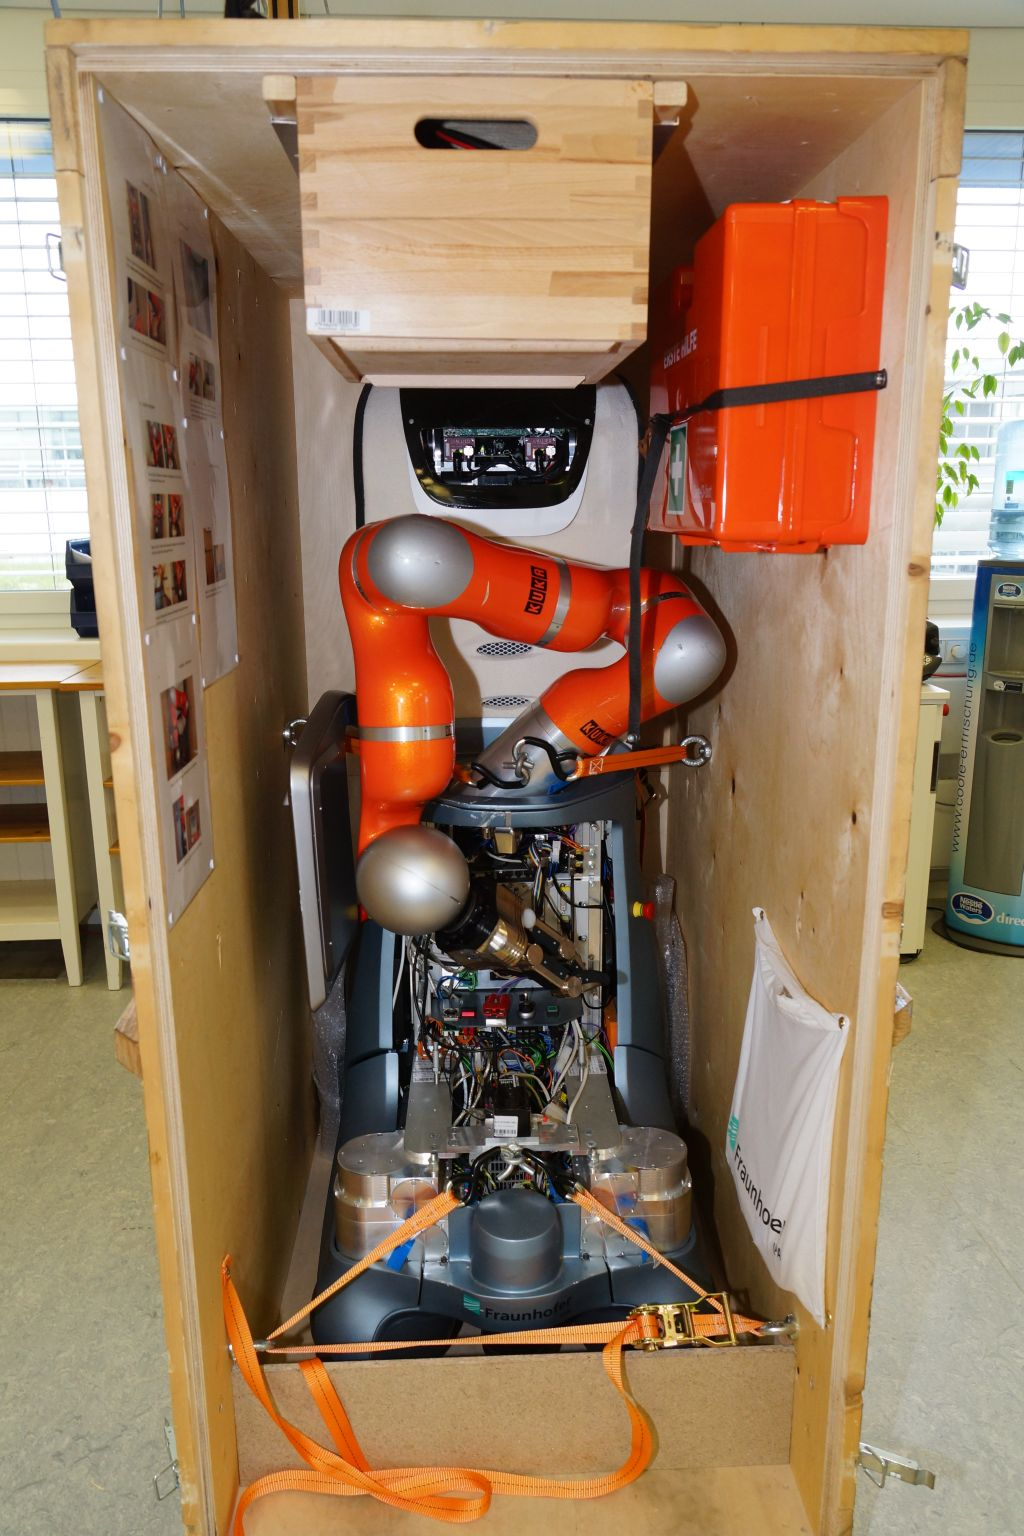
\includegraphics[width=6cm,angle=0]{images/packing_14.jpg} }}
\caption{Step 6: Pack the accessory box as shown (left) and place it in the rails (right).} % \label{fig12} 
\end{figure}

\begin{figure}[!ht]
\centering
\mbox{\subfigure{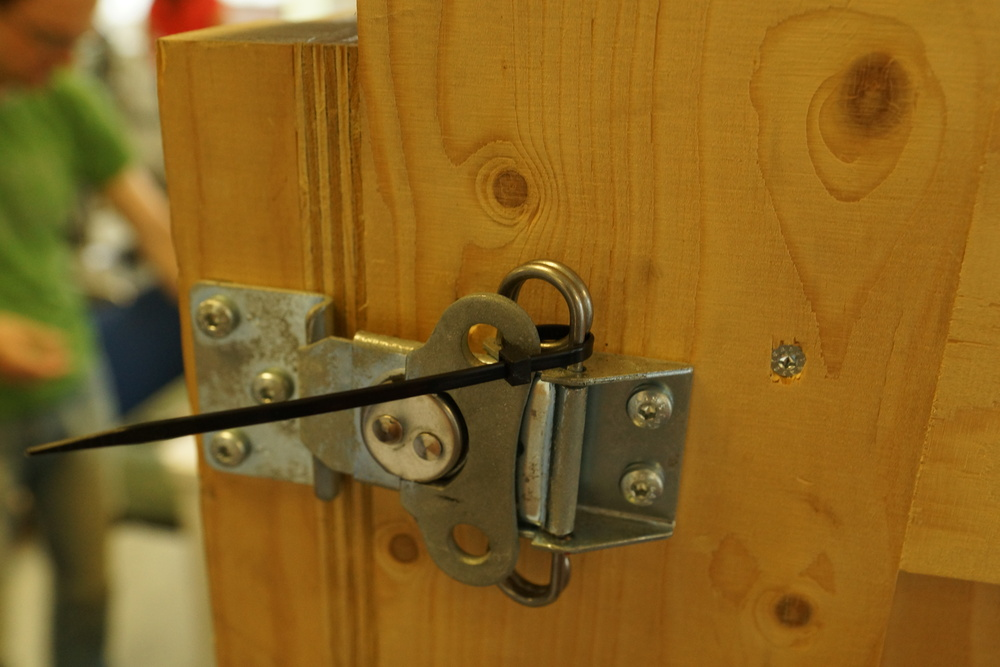
\includegraphics[width=6cm]{images/packing_20.jpg}}\quad
\subfigure{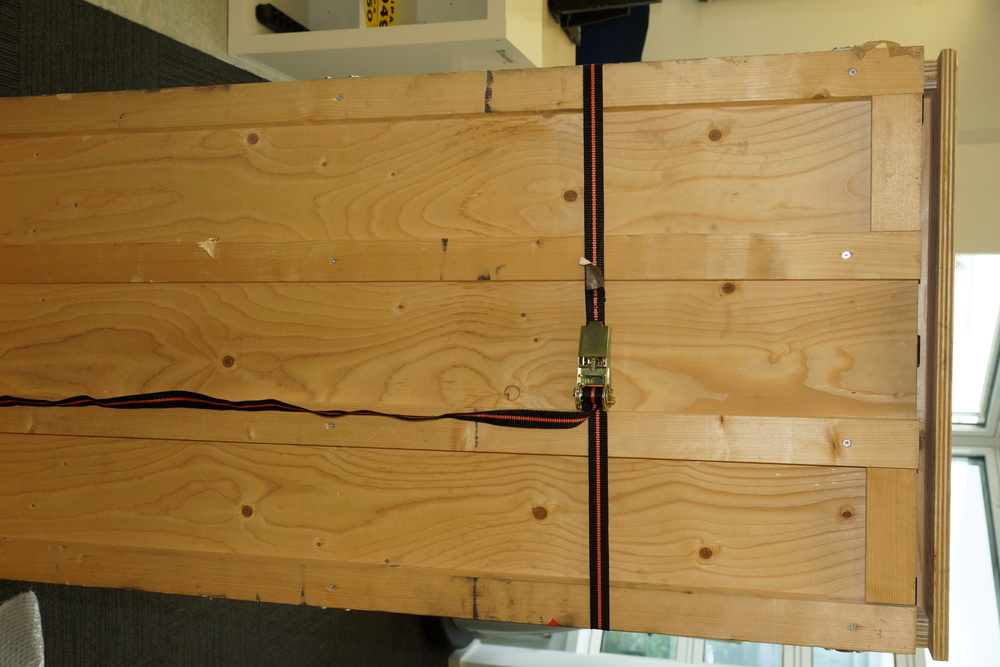
\includegraphics[width=7cm,angle=90]{images/packing_21.jpg} }}
\caption{For air travel, also fix an additional tension belt around the box (left), and seal the hinges with a plastic seal (right).} % \label{fig12}
\end{figure}
